\documentclass[a4paper, 12pt]{article}

\usepackage{listings}
\usepackage{color}
\usepackage[frenchb]{babel}
\usepackage[utf8]{inputenc}
\usepackage[T1]{fontenc}
\usepackage{lmodern}
\usepackage{graphicx}
% Numbers and units
\usepackage[squaren, Gray]{SIunits}
\usepackage{sistyle}
\usepackage[autolanguage]{numprint}
\usepackage{fullpage}
\usepackage[margin=0.7in]{geometry}
\usepackage{multirow}
\usepackage{xparse}
\usepackage{tikz}
\setlength{\parskip}{1em}
\usetikzlibrary{arrows, decorations.markings}

\newcommand\si[2]{\numprint[#2]{#1}}
\newcommand\np[1]{\numprint{#1}}

\newcommand\figref[1]{figure~\ref{fig:#1}}

\NewDocumentEnvironment{myfig}{mm}
{\begin{figure}[!ht]\centering}
{\caption{#2}\label{#1}\end{figure}}

\usepackage[Conny]{fncychap}

\usepackage{enumerate}

\lstset{ %
  backgroundcolor=\color{white},   % choose the background color; you must add \usepackage{color} or \usepackage{xcolor}
  basicstyle=\footnotesize,        % the size of the fonts that are used for the code
  breakatwhitespace=false,         % sets if automatic breaks should only happen at whitespace
  breaklines=true,                 % sets automatic line breaking
  captionpos=b,                    % sets the caption-position to bottom
  commentstyle=\color{mygreen},    % comment style
  deletekeywords={...},            % if you want to delete keywords from the given language
  escapeinside={\%*}{*)},          % if you want to add LaTeX within your code
  extendedchars=true,              % lets you use non-ASCII characters; for 8-bits encodings only, does not work with UTF-8
  frame=single,                    % adds a frame around the code
  keywordstyle=\color{blue},       % keyword style
  language=Java,                   % the language of the code
  morekeywords={*,...},            % if you want to add more keywords to the set
  numbers=left,                    % where to put the line-numbers; possible values are (none, left, right)
  numbersep=5pt,                   % how far the line-numbers are from the code
  numberstyle=\tiny\color{mygray}, % the style that is used for the line-numbers
  rulecolor=\color{black},         % if not set, the frame-color may be changed on line-breaks within not-black text (e.g. comments (green here))
  showspaces=false,                % show spaces everywhere adding particular underscores; it overrides 'showstringspaces'
  showstringspaces=false,          % underline spaces within strings only
  showtabs=false,                  % show tabs within strings adding particular underscores
  stepnumber=1,                    % the step between two line-numbers. If it's 1, each line will be numbered
  stringstyle=\color{mymauve},     % string literal style
  tabsize=2,                       % sets default tabsize to 2 spaces
  columns=flexible,
  title=\lstname                   % show the filename of files included with \lstinputlisting; also try caption instead of title
}

\title{Formalizing Refactorings with Graph Transformation}
\author{Paulus Alois}

\begin{document}

\maketitle

\tableofcontents

\newpage

\section{Introduction}

Qu'est ce que le refactoring ? 

Le refactoring permet de changer la structure d'un programme en vue de l'améliorer
tout en préservant son comportement. 

Le refactoring est généralement appliqué sur des programmes écrit en language orienté objet. Il permet de déplacer certaines fonctionnalités d'une classe à une autre, de renomer des variables à travers tout un programme, ect. Il est utile pour éviter la répétition de code.

Il peut être éffectué à la main. Le programmeur va analyser le code et identifier des parties de code à modifier. Il va ensuite apporter les modifications necessaires.
Cette technique est malheureusement assez lente et peu sure, en effet le programmeur peu faire des erreurs et introduire des bugs.

Pour pallier à ces problèmes, des outils de refactoring sont disponibles et permettent d'automatiser les actions comme le renomage d'une variable, le déplacement d'un fonction ect. Tout en garantissant une certaine sécurité.

Ces outils ne sont malheureusement pas parfait. Ils sont pour la plupart spécialisé dans un seul language de programmation et ne garantisent pas à 100 pourcent la préservation du comportement du programme après un refactoring.

Dans le but de pallier à ces manques, cet article va présenter un moyen de représenter le refactoring comme des transformations de graph. Ces transformations seront vérifiables mathématiquement, ce qui garantira la conservation de certaines propriété du programme.

Ainsi nous auront la possibilité de refactorer en étant certain de ne pas altérer les fonctionnalités de notre programme.

\newpage 

\section{Représentation en graph}
Pour représenter la syntaxe d'un programme orienté objet et les règles de refactoring nous aurons besoin de plusieurs type de graph:

\begin{itemize}
\item Les graphs de type
\item Les graphs de programme
\item Les graphs d'expression
\end{itemize}

En vue de pouvoir s'integrer au mieux dans les logiciels de refactoring, la représentation en graph doit être le plus proche possible d'un arbre de syntaxe abstrait augmanté de lien.

Le model doit rester compréhensible, il est donc important qu'il soit le plus petit possible, de ce faite nous incluerons uniquement les choses utiles aux propriété du refactoring dans le graph.

\subsection{Les différents type de graph}

\subsection{Le graph de type}

Le graph de type sert à spécifier les différentes contraintes qu'un graph de programme devra respecter. Si un graph de programme ne respecte pas toutes les contraintes, il n'est pas syntaxiquement correcte.
Il est indispensable d'établir un graph de type pour prouver que le refactoring produit des programmes avec une syntaxe correcte.

Le graph de type à lui tout seul ne suffit pas à représenter toutes les contraintes, il faut également un ensemble de sous graph interdit.

\begin{enumerate}
\item une classe ne peut pas contenir plusieurs variables avec le même nom
\item une classe ne peut pas contenir plusieurs méthode avec la même signature
\item une expression contenue dans une méthode ne peut pas accéder à des variables contenues dans les descendants de la classe
\item une expression contenue dans une méthode ne peut pas accéder à un paramètre appartenent à une autre méthode.
\end{enumerate}

Malheureusement cet ensemble de graph interdit peut être infini, pour régler ce problème nous auront besoin des graphs d'expression expliqué ci dessous.\label{subsec:graphExpression}

Dans la figure~\ref{typeGraph} se trouve toutes les relations possible entre les nodes en fonction de leur type.
On peut aussi observer quelque cardinalité comme le maximum 1 d'une même définition de méthode dans une classe.

\begin{myfig}{typeGraph}{Graph de type}
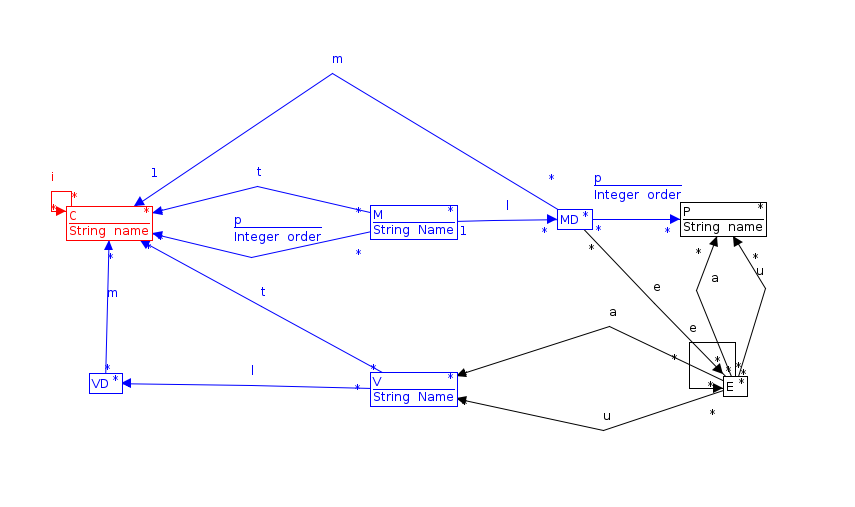
\includegraphics[width=\textwidth]{typeGraph.png}
\end{myfig}

\subsubsection{Les differents type de node}


  \begin{tabular}{ | l | l | l | p{5cm} |}
    \hline
    type & description  \\ \hline
    C & Class   \\ \hline
    M & Signature de méthode   \\ \hline
    MD &  Définition d'une méthode   \\ \hline
    V &  Variable   \\ \hline
    VD &  Définition d'une variable \\ \hline
    P & Paramètre \\ \hline
    E &  Expression contenue dans une définition de méthode \\ \hline

    \end{tabular}

\subsubsection{Les différents type d'arrêtes}

  \begin{tabular}{ | l | l |  l |}
    \hline type & application & description  \\ \hline
    l : & M -> MD & \\ & V -> VD & lookup d'une variable ou d'une méthode à sa définition  \\ \hline 
    i : & C -> C &  héritage d'une classe à une autre de méthode    \\ \hline
    m : & VD -> C & \\ & MD -> C & apartenance d'un variable ou d'une méthode à une classe    \\ \hline
    t : & V -> C  & \\ &  M -> C & type d'une variable ou type de retour    \\ \hline
    p : & MD -> P  & \\ &  P -> C & définition d'un paramètre ou de son type     \\ \hline
    e : & E -> M & expression contenue dans une définition de méthode ou \\ & &  dans une expréssion    \\ \hline
    a : & E -> {V|P} & accèss à une variable ou à un paramètre    \\ \hline
    u : & E -> {V|P} & mise à jour d'une variable ou d'un paramètre    \\ \hline
   \end{tabular}


\subsection{Les graphs de programme} 

Graph typé et labelé (directes) représentant un programme. Il est composé de node reliées entre elle par des arrêtes. Ces nodes et arrêtes prennent les valeurs vu ci dessus dans le graph de type agrémentées de leurs nom ou d'autres attributs.

\subsubsection{Definition}
G composé d'un ensemble de node labelée et d'edge labelée est un graph formé de 3-tuple(Vg,Eg,nlabg) ou Vg est un ensemble de nodes, nlabg: est une function de nomage de node et Eg est un ensemble
d'arrêtes.

Dans un graph de programme les entité (classes, variables, méthodes et paramètres) sont représentés par des nodes dont le label est une paire composée de son nom et de son type.

Les relations entre ces différentes entités (héritage, appelle de méthodes, appartenance) sont représentées par des arrêtes. 
Ces arrêtes possèdes un label pour permettre de faire la différence entre les arrêtes de même type ayant la même source et la même destination.

\begin{myfig}{typedGraph}{Graph du programme Transport}
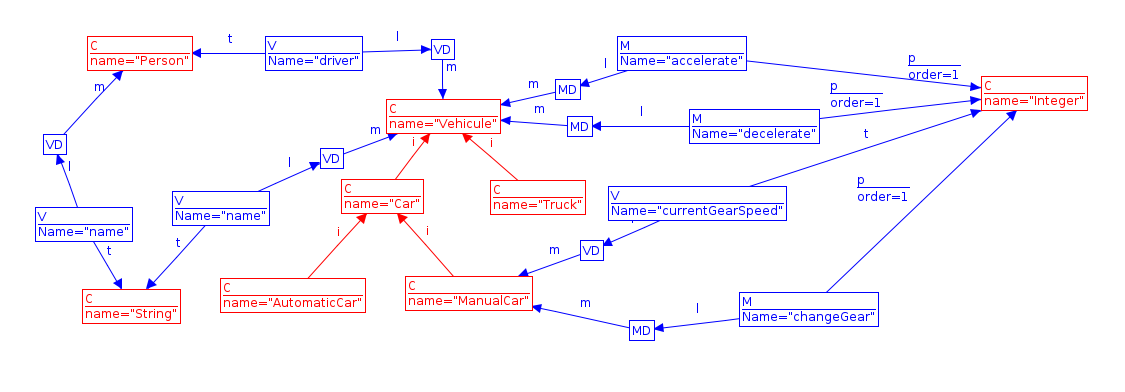
\includegraphics[width=\textwidth]{typedGraph.png}
\end{myfig}

\subsection{Les graph d'expression} 

Dans la section~\ref{subsec:graphExpression} nous avons évoqué les graphs d'expression. Ces graphs dont les labels des arrêtes peuvent être des expressions régulières, permetent de représenter un ensemble de graph à partir d'un seul. Il suffit de remplacer les expressions régulières par leurs valeurs possibles.

\begin{myfig}{graphExpression}{Graph d'expression}
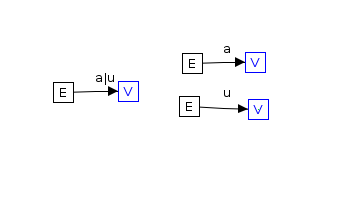
\includegraphics{graphExpression.png}
\end{myfig}

A la gauche de la figure~\ref{graphExpression}, se trouve un graph avec une arrêtes dont le label est une expression régulières. A sa droite sont représenté les deux graphs possible issu du premier graph.

L'exemple reste içi assez simple mais vous pouvez imaginer un graph qui peut representer des centaines d'autres graphs.

\newpage
\section{Programme exemple}

Durant tout l'article, ce programme servira de base aux exemples et aux démonstrations.

C'est un programme simple contenant de l'héritage entre les classes, utile pour PullUpMethod et des attributs utile pour EncapsulateVariable.

\subsection{Vehicules}

\begin{lstlisting}[frame=single]
public class Vehicule {
	public String name;
	public Person driver;

	public void accelerating(int amount) {

	}

	public void decelerate(int amount) {
	
	}
}

public class Truck extends Vehicule {

}

public class Person {
	public String name;
}

public class ManualCar {
	public int currentGearSpeed;
	
	public void changeGear(int number) {
	}
}

public class Car extends Vehicule {

}

public class AutomaticCar {

}
\end{lstlisting}

\newpage
\section{Refactoring}

\subsection{Preservation du comportement}
\label{subsec:preservationDuComportement}
La conservation du comportement d'un programme est une chose primordiale lors d'un refactoring. Cela consiste, en simplifiant, que le programme effectuera les mêmes actions avant et après le refactoring. Nous nous concentrerons ici sur trois proprieté :

\begin{itemize}
\item Preservation de l'accès, chaque méthode accédera au moins à toutes les variables qu'elle accédait avant le refactoring
\item Preservation de la mise à jour, chaque methode mettera à jour au moins toutes les variables mise à jour avant le refactoring
\item Preservation de l'appele, chaque methode appelera au moins toutes les méthodes appelées avant le refactoring
\end{itemize}

\subsection{Encapsulate Variable}

Encapsuler une variable dans une classe est une opération souvent éffectué par les programmeurs. 
Elle consiste à rendre une variable public, privée et à ajouter un accesseur public et un setter public pour continuer à pouvoir accéder et à mettre à jour cette variable.

Lors d'un refactoring cela consiste à changer la visibilité de la variable et à créer deux nouvelles methodes. Ensuite il faut changer tout les accès ou/et mise à jour de la variable par des appels aux deux méthodes crées.

\subsubsection{Condition}

- Il faut que les deux nouvelles méthodes crées ne soit pas déjà présente dans la classe ni dans ses ancêtres et/ou descendants.

WF-1 est préserver car on ne crée ni ne bouge aucune variable.
WF-2 est préserver car la condition stipules qu'ils ne faut pas que des méthodes comportant les même définition que le getter ou le setter soient présente.
WF-3 est préservée car on crée deux méthodes accédant une variable dans la même classe.
WF-4 est préservée car le paramètre de la méthodes setter est employée uniquement dans la définition de cette méthode.

\subsubsection{Avant}

\begin{lstlisting}[frame=single]
public class Person {
	public String name;
}
\end{lstlisting}

\subsubsection{Après}

\begin{lstlisting}[frame=single]
public class Person {
	private String name;
	
	public String GetName(){
		return name;
	}

	public void SetName(String n){
		name=n;
	}
}
\end{lstlisting}

\subsubsection{Représentation graphique}

\begin{myfig}{beforeEncapsulateVariable}{Before Encapsulate Variable}
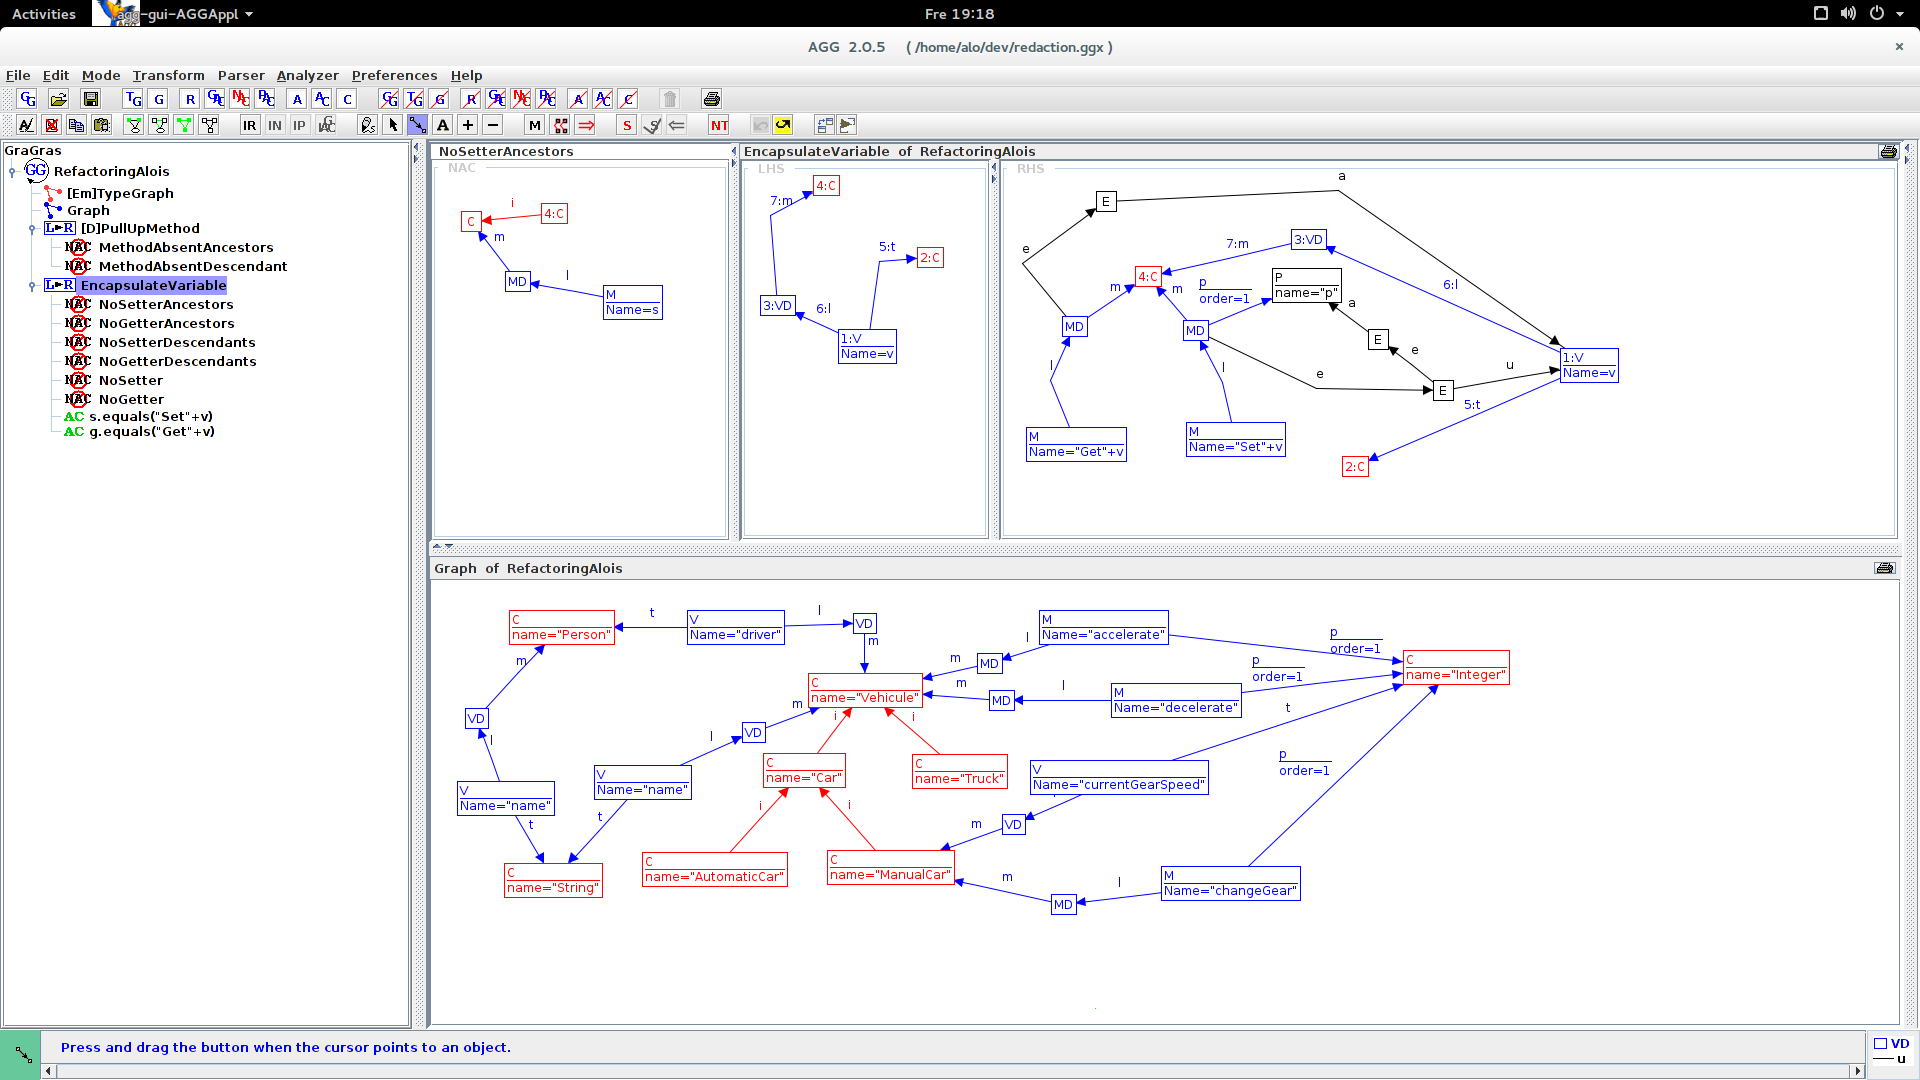
\includegraphics[width=\textwidth]{beforeEncapsulateVariable.png}
\end{myfig}

Dans le haut de la figure~\ref{beforeEncapsulateVariable} se trouve la LHS qui représente la structure d'un sous graph du programme avant sa transformation. A droite, nous avons RHS qui représente la structure de ce sous graph après la transformation. Et en dessous nous avons le graphique du programme.

\begin{myfig}{afterEncapsulateVariable}{After Encapsulate Variable}
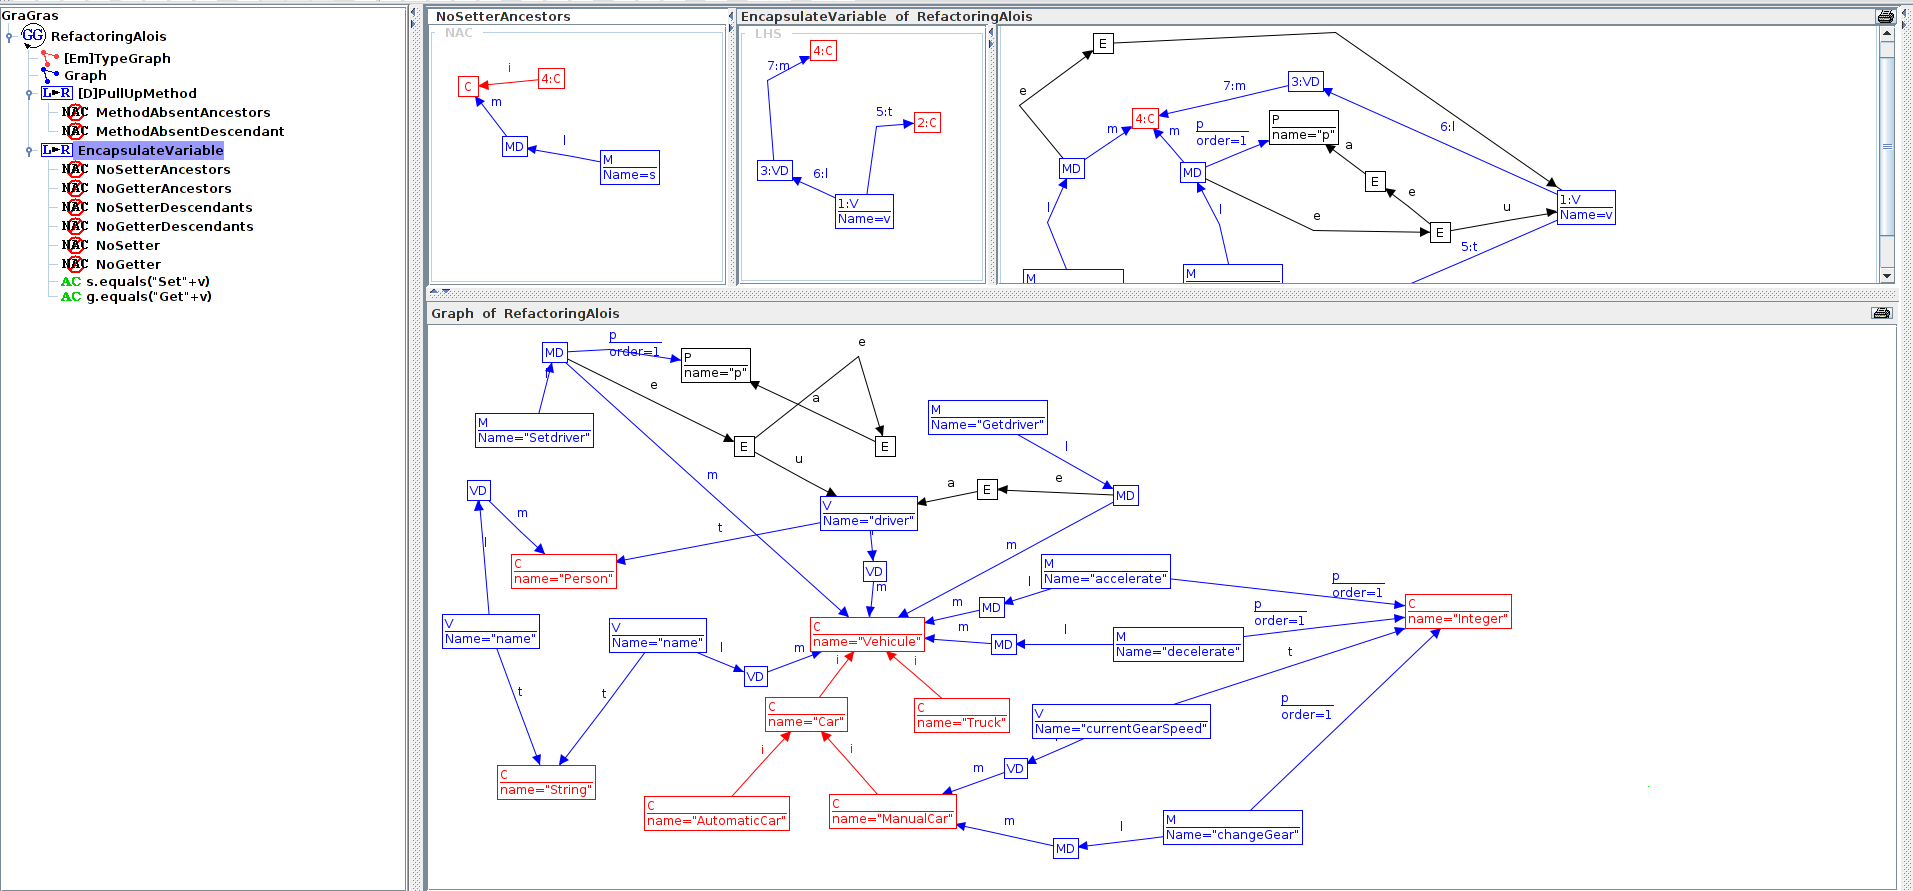
\includegraphics[width=\textwidth]{afterEncapsulateVariable.png}
\end{myfig}

Ici dans la figure~\ref{afterEncapsulateVariable} nous avons les mêmes éléments au dessus mais la partie inférieur à changer. 
Elle représente le graphique après l'application de la transformation.

Je n'ai laisser que la transformation du sous graph lié à la variable "driver" pour une meilleure visibilité. 

Normalement cette transformation s'applique à tout les sous graphs correspondant.

\newpage 

\subsection{Pull Up Method}

Cela consiste à déplacer une méthode présente dans une ou plusieur classes enfant dans la classe parent. 

\subsubsection{Condition}
Les conditions sont:

- La classe parent ne peut pas déjà contenir une méthode ayant la même signature
- Aucune des variables directement accédée ou modifiée par la méthode ne peut être en dehors du scope de la classe parent.

WF-1 est préserver car on ne crée ni ne bougeons aucune variable.
WF-2 est préserver grâce à la précondition qui stipule qu'il ne peut pas se trouver une méthode avec la même signature dans la classe parent.
WF-3 est préservée grâce à la précondition qui stipule que la définition de la méthode bougée ne doit pas accéder à des variables en dehors du scope du parent.
WF-4 est préservée car on ne crée ni ne modifie aucune méthode.

\subsubsection{Avant}
\begin{lstlisting}[frame=single]
public class Vehicule {
	public String name;
	public Person driver;

	public void accelerating(int amount) { 
	}

	public void decelerate(int amount) { 
	}
}

public class Car extends Vehicule {

}

public class ManualCar extends Car {
	public void changeGear(int speed){ 
	}
}
\end{lstlisting}

\subsubsection{Après}
\begin{lstlisting}[frame=single]
public class Vehicule {
	public String name;
	public Person driver;

	public void accelerating(int amount) {

	}
	public void decelerate(int amount) { 
	}
	
	public void changeGear(int speed){
	}
}

public class Car extends Vehicule {

}

public class ManualCar extends Car {

}
\end{lstlisting}

\subsubsection{Représentation graphique}

\begin{myfig}{beforePullUpMethode}{Before PullUp Methode}
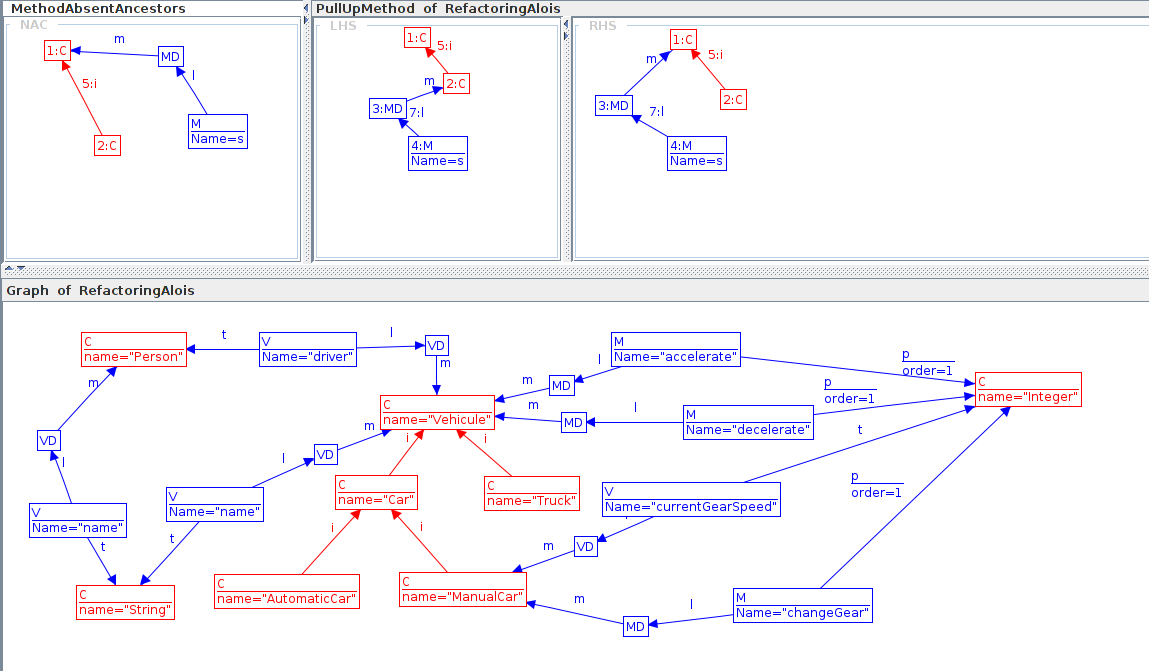
\includegraphics[width=\textwidth]{beforePullUpMethode.png}
\end{myfig}

En haut à gauche de la figure~\ref{beforePullUpMethode} se trouve la LHS qui représente la structure d'un sous graph du programme avant sa transformation. 
En haut à droite de la figure~\ref{beforePullUpMethode} se trouve la RHS qui représente la structure de ce sous graph après la transformation.
En dessous nous avons le graphique du programme.

\begin{myfig}{afterPullUpMethod}{After PullUp Methode}
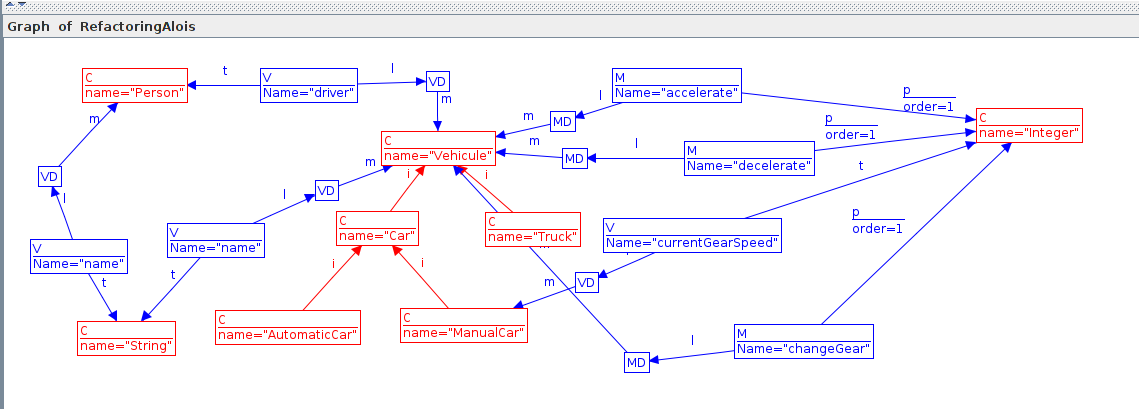
\includegraphics[width=\textwidth]{afterPullUpMethod.png}
\end{myfig}

Dans la figure~\ref{afterPullUpMethod} la partie du dessous à changé et représente le programme après avoir appliqué la transformation en d'autre termes, après avoir remonté la méthode de la classe ManualCar à Vehicule.
Cette méthode a bien été supprimée de la classe ManualCar car il n'existe plus de lien vers celle çi.

\section{Les productions de graph pour exprimer le refactoring}

Comme vu dans les exemples ci dessous, pour exprimer un refactoring on applique des productions de graph sur le graph de programme.

Il reste cependant quelques problèmes:

- Certain type de refactoring modifie une partie, variable, d'un programme ce qui les rend impossible à représenter grâce à une simple production graphique. Il faut donc appliquer plusieurs productions l'une après l'autre dans un ordre spécifique, pour cela nous auront besoin d'un mecanisme de réecriture de graph controllé.

- La representation d'un refactoring devra être sous forme générique et pas spécifique à certains noms de classe ou de methodes du programme sur lequel il est appliqué. Une technique de production de graph avec des paramètres va donc être emloyée.

- Il est possible que certaines arrêtes deviennent orphelines car elle accedait à une variable qui est maintenant uniquement accessible par un getter ou un setter. Ces arrêtes orphlines ne sont normalement pas autorisé dans un graph, mais les éviter serait beaucoup trop complexe. C'est pour cela que l'on emploie un méchanisme "embedding mechanism" qui autorise ces edges orphiles.

\subsection{Définition des règles de transformation de graph}

Pour définir ces règles j'ai préféré utiliser des représentations graphiques.

Quelques notions doivent être définie avant de pouvoir appliquer une production à un graph:

1) G étant un graph, un sous graph de G contient un ensemble de noeud de G et uniquement les arrêtes reliant des noeuds contenu dans ce sous graph. 

2) Quand on applique un mapping sur les noeuds de G, on applique automatiquement un mapping sur les arrêtes reliant ces noeuds.

3) G et K étant des graphs, un occurence de K dans G est très restrictive c'est à dire que que toutes les arrêtes entre les noeuds correspondant doivent exister. 
Voir figure~\ref{sousGraph} 

\tikzstyle{weight} = [font=\small]
\tikzstyle{edge} = [draw,line width=2pt,-,black]
\tikzstyle{vertex}=[circle,fill=black!25,minimum size=10pt,inner sep=0pt]
\begin{myfig}{sousGraph}{Exemple sous graph}
\begin{tikzpicture}[scale=1.8, auto,swap]
    % Draw a 7,11 network
    % First we draw the vertices
    \foreach \pos/\name in {{(0,2)/b}, {(2,2)/c}, {(1,1)/e},
                            {(0,0)/a}, {(2,0)/d}}
        \node[vertex] (\name) at \pos {$\name$};
    % Connect vertices with edges and draw weights
    \foreach \source/ \dest /\weight in {a/b/1, c/b/2,c/d/3,d/a/4,
                                         e/c/5, b/e/6}
        \path[edge] (\source) -- node[weight] {$\weight$} (\dest);

\end{tikzpicture}
\end{myfig}



\begin{myfig}{sousGraph}{Exemple sous graph valide}
\tikzstyle{edge} = [draw,line width=2pt,-,green]
\tikzstyle{vertex}=[circle,fill=green!25,minimum size=10pt,inner sep=0pt]
\begin{tikzpicture}[scale=1.8, auto,swap]
    % Draw a 7,11 network
    % First we draw the vertices
    \foreach \pos/\name in {{(0,2)/b}, {(2,2)/c}, {(1,1)/e}}
        \node[vertex] (\name) at \pos {$\name$};
    % Connect vertices with edges and draw weights
    \foreach \source/ \dest /\weight in {c/b/2,
                                         e/c/5, b/e/6}
        \path[edge] (\source) -- node[weight] {$\weight$} (\dest);
\end{tikzpicture}
\end{myfig}


\begin{myfig}{sousGraph}{Exemple sous graph invalide}
\tikzstyle{edge} = [draw,line width=2pt,-,red]
\tikzstyle{vertex}=[circle,fill=red!25,minimum size=10pt,inner sep=0pt]
\begin{tikzpicture}[scale=1.8, auto,swap]
    % Draw a 7,11 network
    % First we draw the vertices
    \foreach \pos/\name in {{(0,2)/b}, {(2,2)/c}, {(1,1)/e}}
        \node[vertex] (\name) at \pos {$\name$};
    % Connect vertices with edges and draw weights
    \foreach \source/ \dest /\weight in {c/b/2, b/e/6}
        \path[edge] (\source) -- node[weight] {$\weight$} (\dest);
\end{tikzpicture}
\end{myfig}


\subsubsection{Definition}

La définition mathématique est donnée à la page 15 de l'article "Formalizing Refactorings with Graph Transofrmations".

\begin{myfig}{sousGraph}{EMBin et EMBout}
\tikzset{>=latex}
\begin{tikzpicture}
    \node[empty] at (1,5) {L};
    \draw (2,4) ellipse (1cm and 0.5cm);
    \node[empty] at (2,4) {V};

    \draw[->] (5,4) -- +(1,0);
    \draw[->] (2,3) -- +(0,-1) node[anchor=m] {m};

    \node[empty] at (8,5) {R};
    \draw (9,4) ellipse (1cm and 0.5cm);
    \node[empty] at (9,4) {W};

    \draw[->] (9,3) -- +(0,-1) node[anchor=n] {n};

    \node[empty] at (0,1) {G};
    \draw (2,0) ellipse (2cm and 1cm);
    \draw (2,0) ellipse (1cm and 0.5cm);
    \node[empty] at (2,0) {m(v)};

    \draw[->] (5,0) -- +(1,0);

    \draw (3.5,0) node[anchor=south] (e) {\textbullet};
    \draw (2.5,0) node[anchor=south] (f) {\textbullet};

    \draw (0.5,0) node[anchor=south] (g) {\textbullet};
    \draw (1.5,0) node[anchor=south] (h) {\textbullet};
 
   \draw[-latex] (e.west) to[out=90,in=70] (f.east);

   \draw[-latex] (h.west) to[out=70,in=90] (g.east);

    \node[empty] at (7,1) {H};
    \draw (9,0) ellipse (2cm and 1cm);
    \draw (9,0) ellipse (1cm and 0.5cm);
    \node[empty] at (9,0) {n(w)};

    \draw (10.5,0) node[anchor=south] (a) {\textbullet};
    \draw (9.5,0) node[anchor=south] (b) {\textbullet};

    \draw (7.5,0) node[anchor=south] (c) {\textbullet};
    \draw (8.5,0) node[anchor=south] (d) {\textbullet};
 
   \draw[-latex] (a.west) to[out=90,in=70] (b.east);

   \draw[-latex] (d.west) to[out=70,in=90] (c.east);

\end{tikzpicture}

\end{myfig}

Je vais tout de même l'expliquer en français à l'aide de la figure~\ref{sousGraph}.

G et H sont des graphs, m est une fonction de mapping de L vers G et n est une fonction de mapping de R vers H.

m(V) est un sous graph de G et n(w) est un sous graph de H.

{$V_H$} est égale au graph G moins m(v) + n(w), De facon très imagée on peux voir ça comme si on retirais un jaune d'oeuf et on le remplacait par un autre.

Embin est utilisée pour rediriger les arrêtes du reste du graph qui pointais vers des arrêtes contenue dans m(v).
Embout est utilisée pour rediriger les arrêtes contenue dans m(v) qui pointais vers des arrêtes du reste du graph.


\subsection{Pull Up Method}

\begin{myfig}{LHSRHSPullUpMethod}{LHS et RHS}
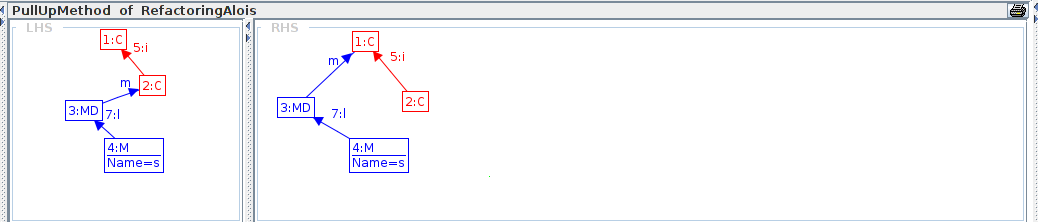
\includegraphics[width=\textwidth]{LHSRHSPullUpMethod.png}
\end{myfig}

\section{Precondition de refactoring}
Pour exprimer les différentes conditions necessaire à un refactoring, il est plus facile d'utiliser des precondition.

Elle servent à définir un sous graph ou un ensemble de sous graph ne pouvant pas être présent avant d'appliquer le refactoring.

\subsection{Pull Up Method}

\begin{myfig}{NACPullUpMethod}{NAC}
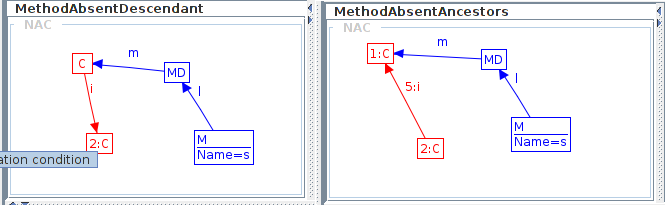
\includegraphics[width=\textwidth]{NACPullUpMethod.png}
\end{myfig}

La figure~\ref{NACPullUpMethod}, représente les deux préconditions nécessaire pour pouvoir appliquer le refactoring PullUpMethod.
Elle spécifie que aucun ancêtre ni descendant de la classe ne possède cette méthode.

\section{Préservation du comportement du programme}

Le but de cette partie est de démontrer que certaines propriétés sont preservée après un refactoring, plus particulièrement les propriété de types, accès à une variable, mise à jour d'un variable et appelle de méthode.

Ces types de comportement introduit dans la sous section~\ref{subsec:graphExpression} 
Pour prouver cela il faut prouver que si une expression existe avant un refactoring, il existe une expression correspondante après. 

Par exemple, chaque définition de méthode qui met à jour une variable dans un graph de départ, doit mettre à jour cette variable dans le graph résultat.

MD ( e|c ) * a -> V -> VD

\subsection{Préservation du comportement : Encapsulate Variable}

On peut observer ici que la mise à jour de la variable dans une méthode est conservée après le refactoring, la seule différence est que l'on appéle une méthode qui met à jour la variable à la place de
dirrectement mettre à jour la variable. Ce qui a comme résultat que le chemin de la MD jusqu'à la variable devient plus long


\section{Conclusion}


\end{document}
